\documentclass[titlepage, twocolumn]{article}

\usepackage{color,latexsym,amsmath,amssymb,graphicx, float}
\usepackage{hyperref}
\usepackage{tabularx}
\usepackage{titling}
\usepackage{subcaption}
\graphicspath{{./figures}}

\hypersetup{
colorlinks=true,
linkcolor=magenta,
filecolor=magenta,
urlcolor=cyan,
}

\newcommand{\red}[1]{\textcolor{red}{#1}}
\newcommand{\subtitle}[1]{%
  \posttitle{%
    \par\end{center}
    \begin{center}\large#1\end{center}
    \vskip0.5em}%
}

\begin{document}

\title{Engineering Physics 353 Final Report}
\subtitle{Team 15}
\author{Nathan Van Rumpt, Eric Souder}
\date{April 2023}

\maketitle

\section{Background}

    The final project for Engineering Physics 353 is the creation of ROS packages to control a simulated robot as it attempts to drive around a streetscape - composed of an inner and outer loop - and record license plate numbers off of parked cars. 
    
    \begin{figure}
    \centering
    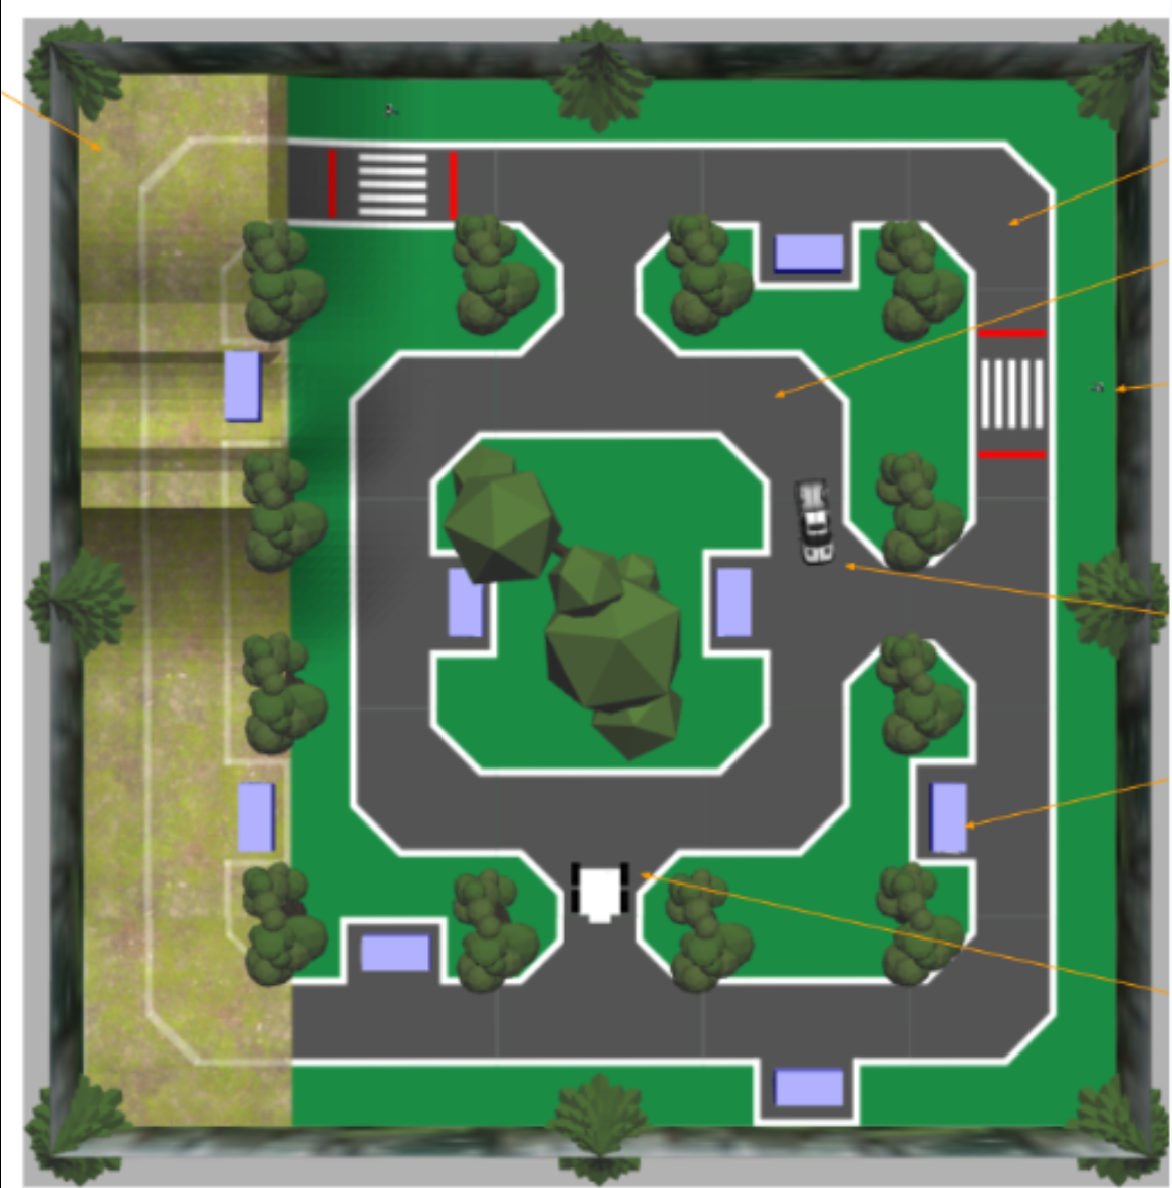
\includegraphics[width=0.7\linewidth]{Competition Space.png}
    \caption{Competition track layout}
    \label{fig:label}
    \end{figure}
    
    The robot must be capable of navigating entirely autonomously while avoiding collisions with pedestrians and other vehicles in the environment. Points were awarded for correctly reporting a license plate over a ROS topic (6 points for plates on the outer ring, and 8 points for plates on the inner ring) and for completing a full lap, and deducted for hitting pedestrians, other cars, or driving off the road. Our team attempted to create a robot that would be primarily capable of very reliably navigating the track and collecting the maximum amount of points. As a secondary objective, we aimed to have the robot complete as quickly as possible, as tie scores would be broken by the robot with the fastest time.

\section{Overall Architecture}

    The robot control software was divided into two ROS packages - one which managed the navigation of the robot and guided it around the track, and one which managed the license plate detection and reporting. The navigation package was composed of a state machine node and a navigation node, which were responsible for controlling the robot's movement around the track, while the plate detection packaged contained a single node responsible for detecting license plates and reporting them over a ROS topic. Additionally, a graphical user interface used for debugging and running the robot was developed and stored in a separate repository. The overall architecture of the robot is shown in Figure~\ref{fig:architecture}. 

    \begin{figure}
        \centering
        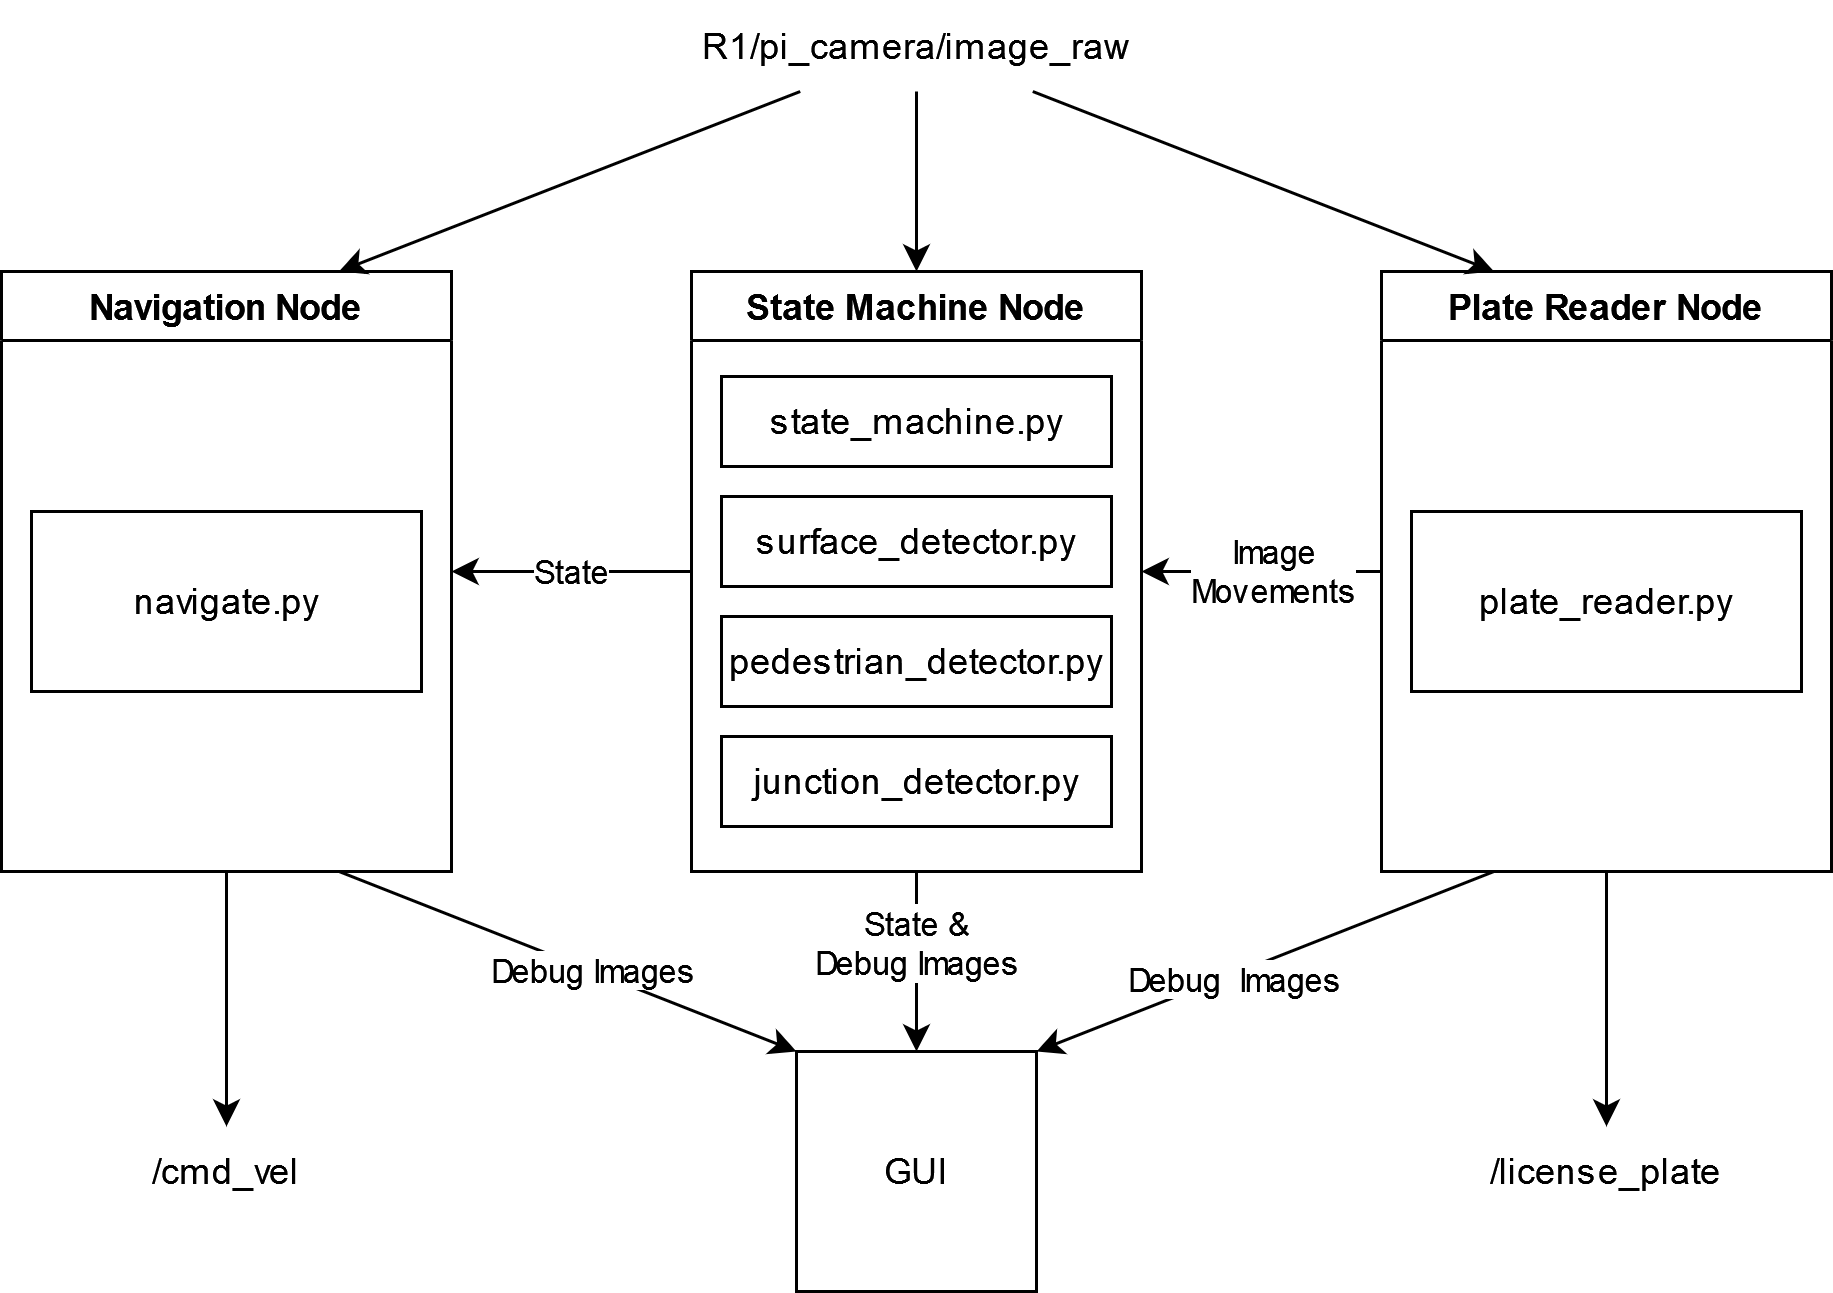
\includegraphics[width=0.8\linewidth]{architecture.png}
        \caption{Overall architecture of the robot control software.}
        \label{fig:architecture}
    \end{figure}
\section{Navigation}
    Robot navigation was accomplished with an almost entirely classical control system, using minimal neural network based approaches and instead using manually tuned computer vision and classical control techniques. 

    The navigation controller was composed of two ROS nodes: The `State Machine' node was composed of a finite state machine and the `Navigate' node contained a set of navigation algorithms for different scenarios, selecting an appropriate algorithm based on the state reported by the state machine. States were communicated internally between the two nodes via a ROS topic.
    
    \subsection{State Machine}
        The finite state machine responsible for controlling the robot's navigation state was composed primarily of a number of state classes, representing a unique navigational state and a state machine class responsible for orchestrating the transitions between them. Each state class, such as the `Pave Navigate' or `Junction Wait' states, is a subclass of an abstract parent class which defines an `evaluate transition' interface responsible for determining the next state to enter and either returns itself (to remain in the current state) or generates a new state object to transition into. 
        
        The state machine class calls this method each frame to determine which state the robot should be in, and then broadcasts that state to the navigation node via a ROS topic. The overall state machine diagram is shown in Figure~\ref{fig:statemachine}.

        \begin{figure}
            \centering
            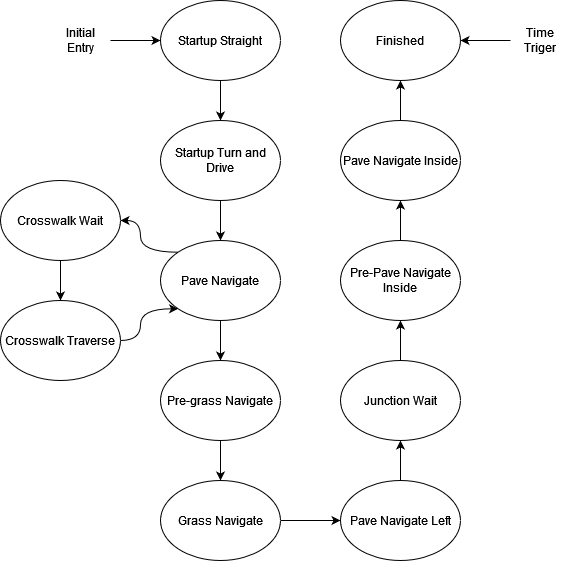
\includegraphics[width=0.8\linewidth]{statemachine.png}
            \caption{Diagram of the robot state machine.}
            \label{fig:statemachine}
        \end{figure}

        Three main types of navigational states existed: active navigation states, stopped states, and preprogrammed states. In preprogrammed states, where the robot executes a constant movement, the state machine transitions based off of a simple timer to move to the next state once the movement had been in progress for the preprogrammed length of time. In active navigation states, where the navigation algorithm is interpreting each frame on the fly to determine a which movement to command, or in stopped states, where the robot is waiting for an event to occur before proceeding, the state machine interprets each frame and makes a transition decision based on it.

        \subsubsection{Pavement and Grass Detection}
            In order to transition from the pavement navigation states to the grass navigation state and vice versa, the state machine must be able to determine if the robot is driving on grass or on pavement. This detection is accomplished with a small neural network, implemented within a `SurfaceDetector' class. Training data was 400 images captured from the robot camera, evenly split between grass and pavement surfaces. 
            
            Data was acquired by manually driving the vehicle around with a simple ROS node activated to save each camera frame. Because of the goal of simplicity for the neural network, all images were preprocessed by significant compression. Images were resized to 0.025 times their original width and 0.05 times their original height. This resulted in a 36 by 32 image, which was further cropped to remove the top 18 rows of pixels, focusing only on the ground and removing the area above the horizon.

            The simple model was composed of only three layers: An input flatten layer, a hidden dense layer, and an output dense layer composed of a single neuron, with a total of 2,666,689 trainable parameters, as shown in Figure~\ref{fig:surfacedetectmodel}.
            \begin{figure}
                \begin{tabularx}{0.9\linewidth}{ 
                     >{\raggedright\arraybackslash}X 
                     >{\raggedright\arraybackslash}X 
                     >{\raggedleft\arraybackslash}X  }

                     Layer (type) & Output Shape & Num. Params. \\ 
                    \hline \\
                    Flatten & (None, 1632) & 0 \\  
                    Dense & (None, 1632) & 2665056 \\
                    Dense & (None, 1) & 1633 \\
                \end{tabularx}
                \caption{Summary of surface detection neural network}
                \label{fig:surfacedetectmodel}
            \end{figure}
            The model was trained with a learning rate of $1 \times 10^{-4}$ and a validation split of 0.2 over 10 epochs. Loss and accuracy curves by epoch are shown in Figure~\ref{fig:grasspavegraphs}.

            \begin{figure}
                \begin{center}
                    \begin{subfigure}{0.5\linewidth}
                        \centering
                        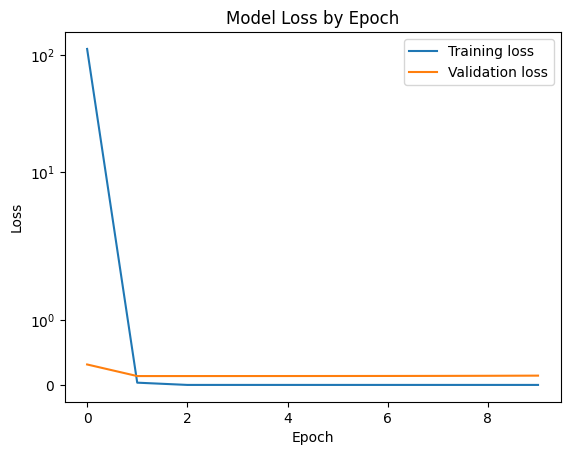
\includegraphics[width=0.9\linewidth]{grasspaveloss.png}
                      \end{subfigure}%
                      \begin{subfigure}{0.5\linewidth}
                        \centering
                        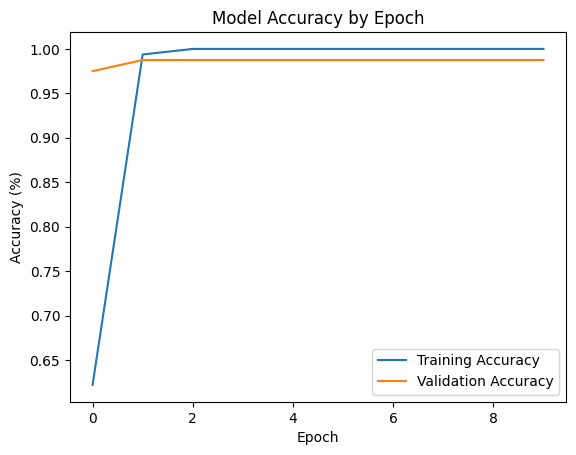
\includegraphics[width=0.9\linewidth]{grasspaveacc.png}
                      \end{subfigure}
                \end{center}
                \caption{Loss and accuracy of grass and pavement detection network by training epoch.}
                \label{fig:grasspavegraphs}
            \end{figure}

            Because of the small size and binary output of the network, little work was deemed necessary to validate it's performance and there was no need for extensive error analysis. A robot was manually driven around the track and the output of the network's predictions was monitored to ensure it was sensible before it was integrated with the state machine to trigger transitions between pavement and grass navigation states.

        \subsubsection{Crosswalk and Pedestrian Detection}
            When navigating over the first section of paved track, two crosswalks with pedestrians must be safely crossed without hitting any pedestrians. The robot must detect the presence of a crosswalk and transition to a `Crosswalk Wait` state in order to avoid hitting a pedestrian. Detection of both crosswalks and pedestrians is performed by methods within the `PedestrianDetector' class. First, crosswalks were detected using simple HSV colour threshold. A crosswalk was considered 'detected' when 1500 total pixels matching the range of colours associated with the red crosswalk stop line were detected in the bottom 100 rows of the image. 
            
            Although 1500 pixels is less than 2 full horizontal rows - much less than the size of the detection area - the need for a large area was the result of the relative high velocity which meant that the robot may only receive one or two frames to detect the crosswalk, so the larger area was chosen as a compromise between guaranteeing detection of the stop line and constantly stopping at around the same location. It also provides detection capability if the line is approached at an angle. This hedges against a possible 10 point loss from hitting a pedestrian of other parts of the navigation system fail.

            Once the crosswalk was detected and the robot was in the `Crosswalk Wait' state, we must detect pedestrians to determine when it is safe to cross. Pedestrians were detected using HSV thresholding to detect their blue jeans, similarly to the crosswalk detection. However, since the location (not just boolean presence) of the pedestrians was needed, erosion and dilation were used to merge the thresholded areas together into fewer, larger `blobs'. The algorithm then finds the contours of each `blob' and selects the largest as the most likely choice to be the pedestrian. Each frame, A bounding box is drawn around it, and its position is found. This process is outlined in Figure~\ref{fig:pants}.

            \begin{figure}
                \centering
                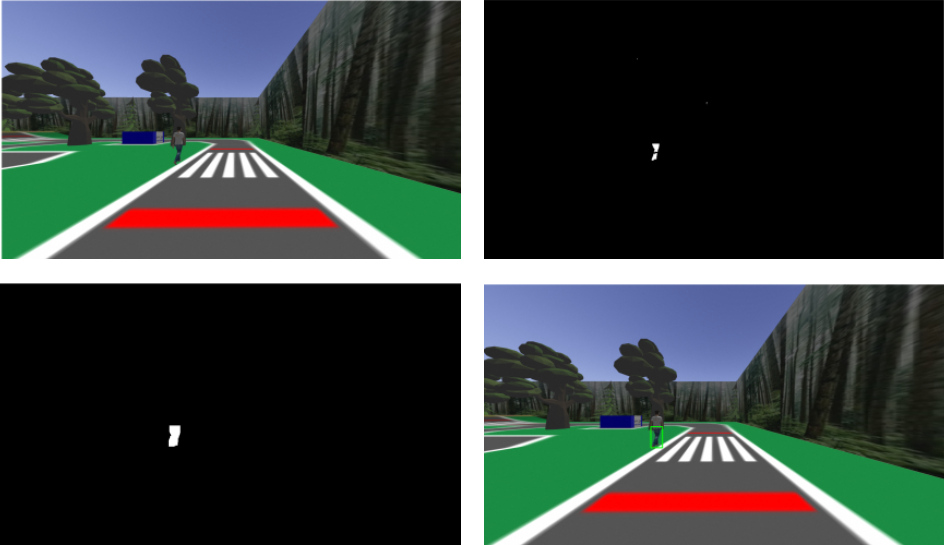
\includegraphics[width=0.8\linewidth]{pants.png}
                \caption{Major steps in pants detection. Left-to-right, top-to-bottom: Input image, HSV thresholding, erosion \& dilation, bounding box.}
                \label{fig:pants}
            \end{figure}

            As a result of the repeatability of our pavement navigation algorithms, the edges of the crosswalk were able to be hard-coded into the pedestrian detector. The state machine tracks the position of the detector, and waits for it to be found in the crosswalk and then to exit the crosswalk. At this point, we can guarantee the maximum amount of time that the pedestrian will not be in the crosswalk, and the state machine is then able to transition to a `Crosswalk Traverse' sprint across the crosswalk before returning to the normal pavement navigation state. 
            
        \subsubsection{Junction and Truck Detection}
            In order to transition to the inner loop of track, the robot must turn through the junction to the inner loop, stop within the junction, wait for the truck to pass safely, and then proceed into the junction. This is accomplished through state transitions using methods with the `JunctionDetector' class.

            When the vehicle exits the grass segment, the state machine switches to the `Pave Navigate Left' mode, tracking the left side of the track rather than the right side as it does for other pavement navigation states. After three seconds of this, the state machine begins attempting to go through a procedure to see if it has reached the junction with the inner track by monitoring the width of the pavement in front of it. 
            
            The pavement width is determined by HSV thresholding to the colour of the pavement and counting the distance between the right- and leftmost valid pixels at a horizontal line 150 pixels up from the bottom of the frame. The algorithm used to evaluate if we are in the junction is shown in Figure ~\ref{fig:junctionalg}, which works by exploiting the characteristic pattern of the pavement appearing to widen, narrow, and then widen again as we turn into the junction, as seen in Figure~\ref{fig:charwidth}. The state machine then transitions to a stopped `Junction Wait' state. 

            \begin{figure}
                \begin{center}
                    \begin{subfigure}{0.5\linewidth}
                        \centering\captionsetup{width=.9\linewidth}%
                        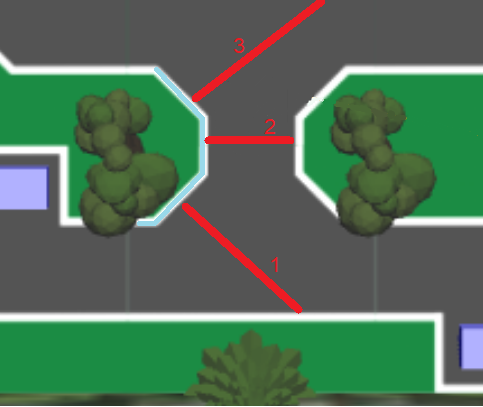
\includegraphics[width=0.9\linewidth]{charwidth.png}
                        \subcaption{Characteristic pattern of widening (1),
                         narrowing (2), and widening again (3)
                          as we follow the inner line.}
                        \label{fig:charwidth}
                      \end{subfigure}%
                      \begin{subfigure}{0.5\linewidth}
                        \centering\captionsetup{width=.9\linewidth}%
                        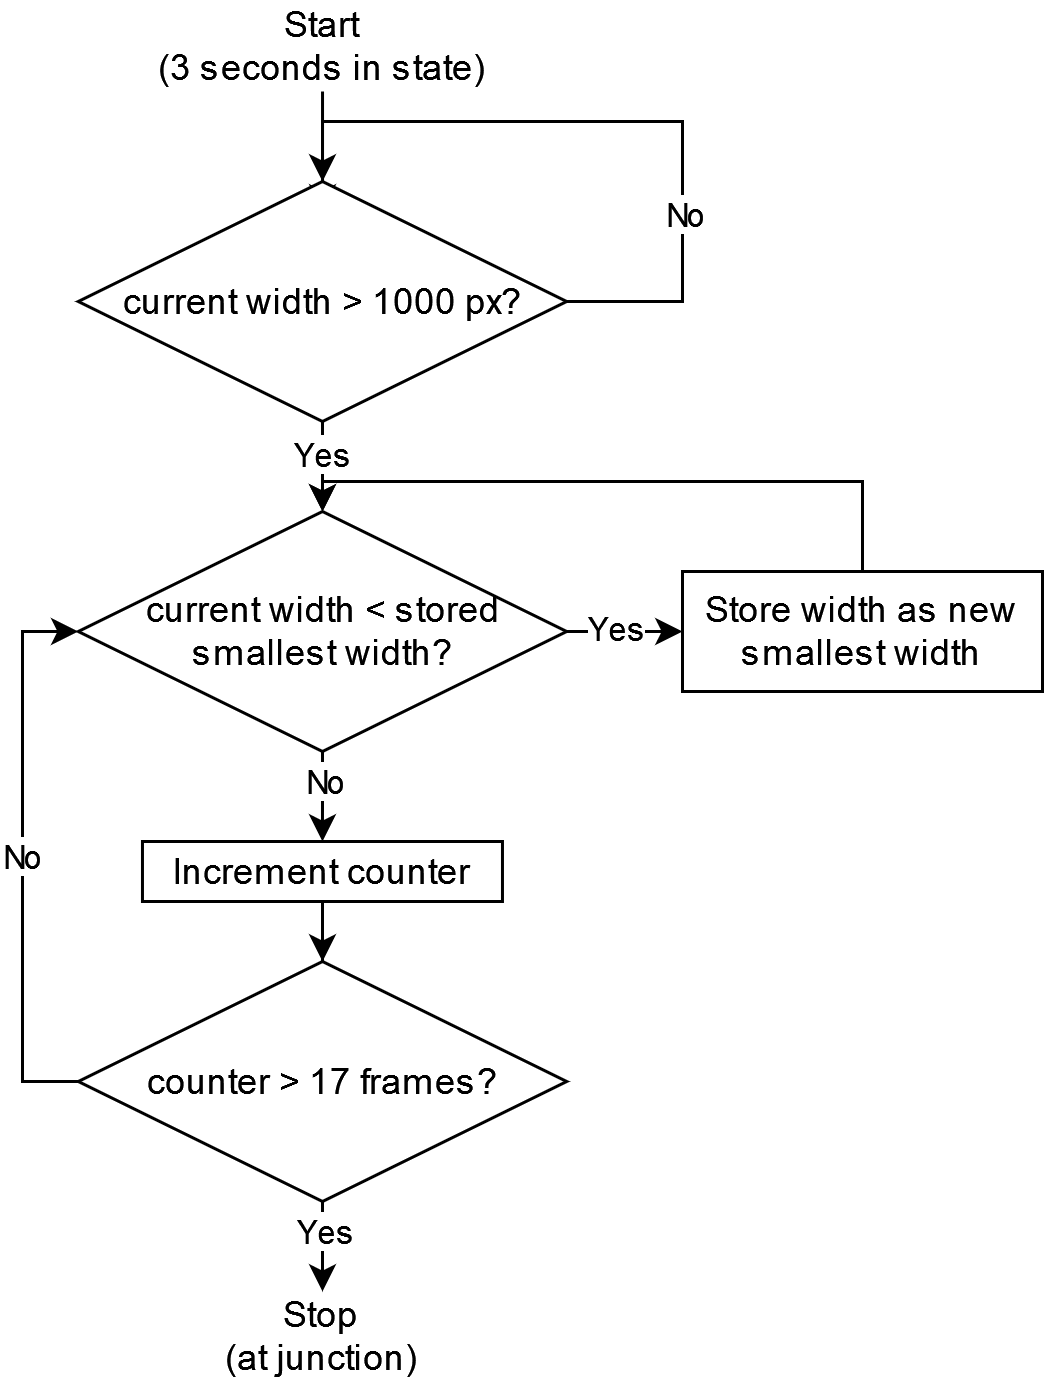
\includegraphics[width=\linewidth]{junctiondiagram.png}
                        \subcaption{Flowchart showing junction detection algorithm based on pavement width.}
                \label{fig:junctionalg}
                      \end{subfigure}
                    \centering\caption{Junction detection algorithm based on pavement width.}
                \end{center}
                \label{fig:junctiondetect}
            \end{figure}

            In the `Junction wait' state, the state machine waits to detect the truck in the appropriate position to safely start the inner loop navigation. Truck detection is based on a very similar methodology as pedestrian pant detection, using HSV colour thresholding followed by erosion, dilation, and contour finding. The state machine will proceed to the next state (moving into the inner loop) once the truck reaches a position in the frame of $x < 400$ pixels and $y<700 $ pixels, a zone that was experimentally determined safe. These values were able to be hard-coded because the position of the robot when waiting at the junction remained extremely consistent throughout runs. 


            
    \subsection{Navigation Algorithms}

        During the active navigation states, the navigation node processes each frame from the camera and uses it to determine a steering angle to publish based on an algorithm tailored for the state it is in. The two main types of active navigation nodes, for paved surfaces and grass surfaces employed relatively similar processes to determine steering angles by attempting to find the edge of the track and hold it at a constant bearing using a proportional controller to determine angular control and holding a constant speed. The main difference between the two was the method used to find the edge of the track.

        \subsubsection{Pavement Navigation}
            
            During pavement navigation, the edge of the track is found through an image processing pipeline to output a binary image with the edge of the track as white pixels and the rest of the image as black pixels. This binary image is then processed to find the center of the track, which is used to determine the steering angle. The image processing pipeline is shown in Figure~\ref{fig:pavepipeline}. The HSV threshold, greyscale, and binary threshold steps convert our frame into a single binary image that we are able to run edge detection and line finding on, while the dilation and erosion steps remove `holes' in the pavement caused by the environment's 1~m grid lines. Sobel edge detection is used to find the edges of the pavement, and then we crop the image to only include the pavement area of interest, ignoring the sky and trees. 
            
            A Hough transform is used to find the lines that best fit the edges, and these lines are then drawn onto a new, blank image which we can then convert to binary and use a simple weighted average to find the centroid of the edge, restricting ourselves to a zone between a certain number of pixels from the bottom of the image - to avoid looking too far into the `future' or focusing too much on lines immediately close to robot - and to either the left or right side of the image depending on if we are navigating based on the left or right side of the track. 

            We navigate based on the right side in almost all pavement areas, as it does not have any junctions interrupting the lines, but on the left side of the track in the `Pave Navigate Left' state, as we want to follow the left line into the junction in order to transition to the inner loop. 

            \begin{figure}
                \begin{center}
                    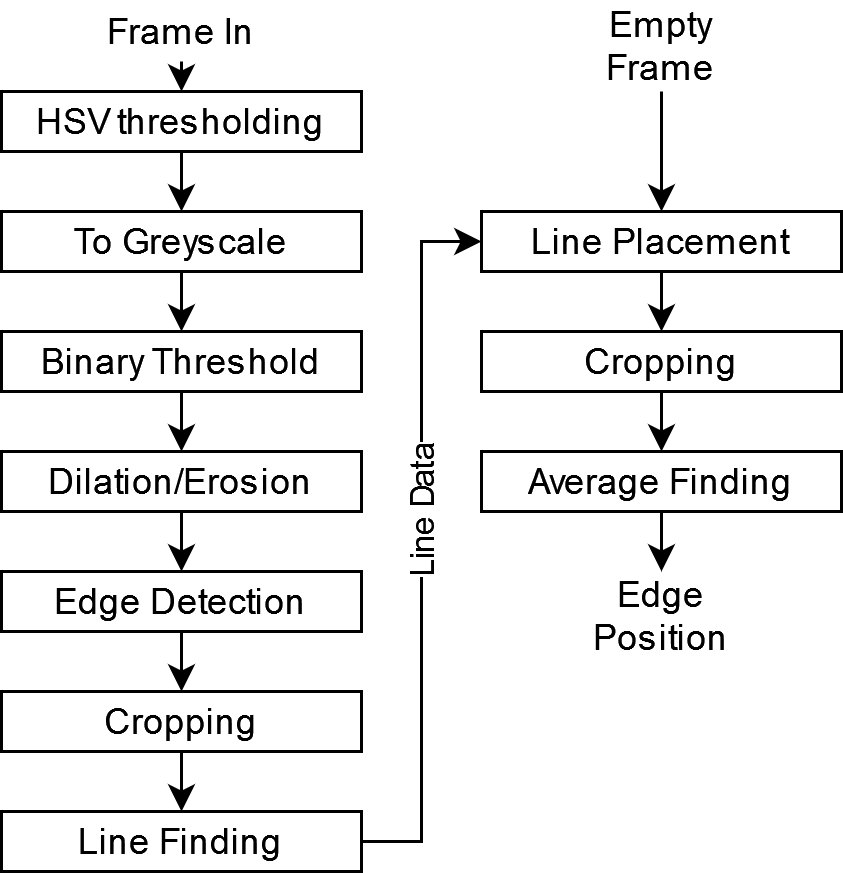
\includegraphics[width=0.6\linewidth]{pavepipeline.png}
                \end{center}
                \caption{Pavement edge detection image processing pipeline.}
                \label{fig:pavepipeline}
            \end{figure}

            \begin{figure}
                \centering
                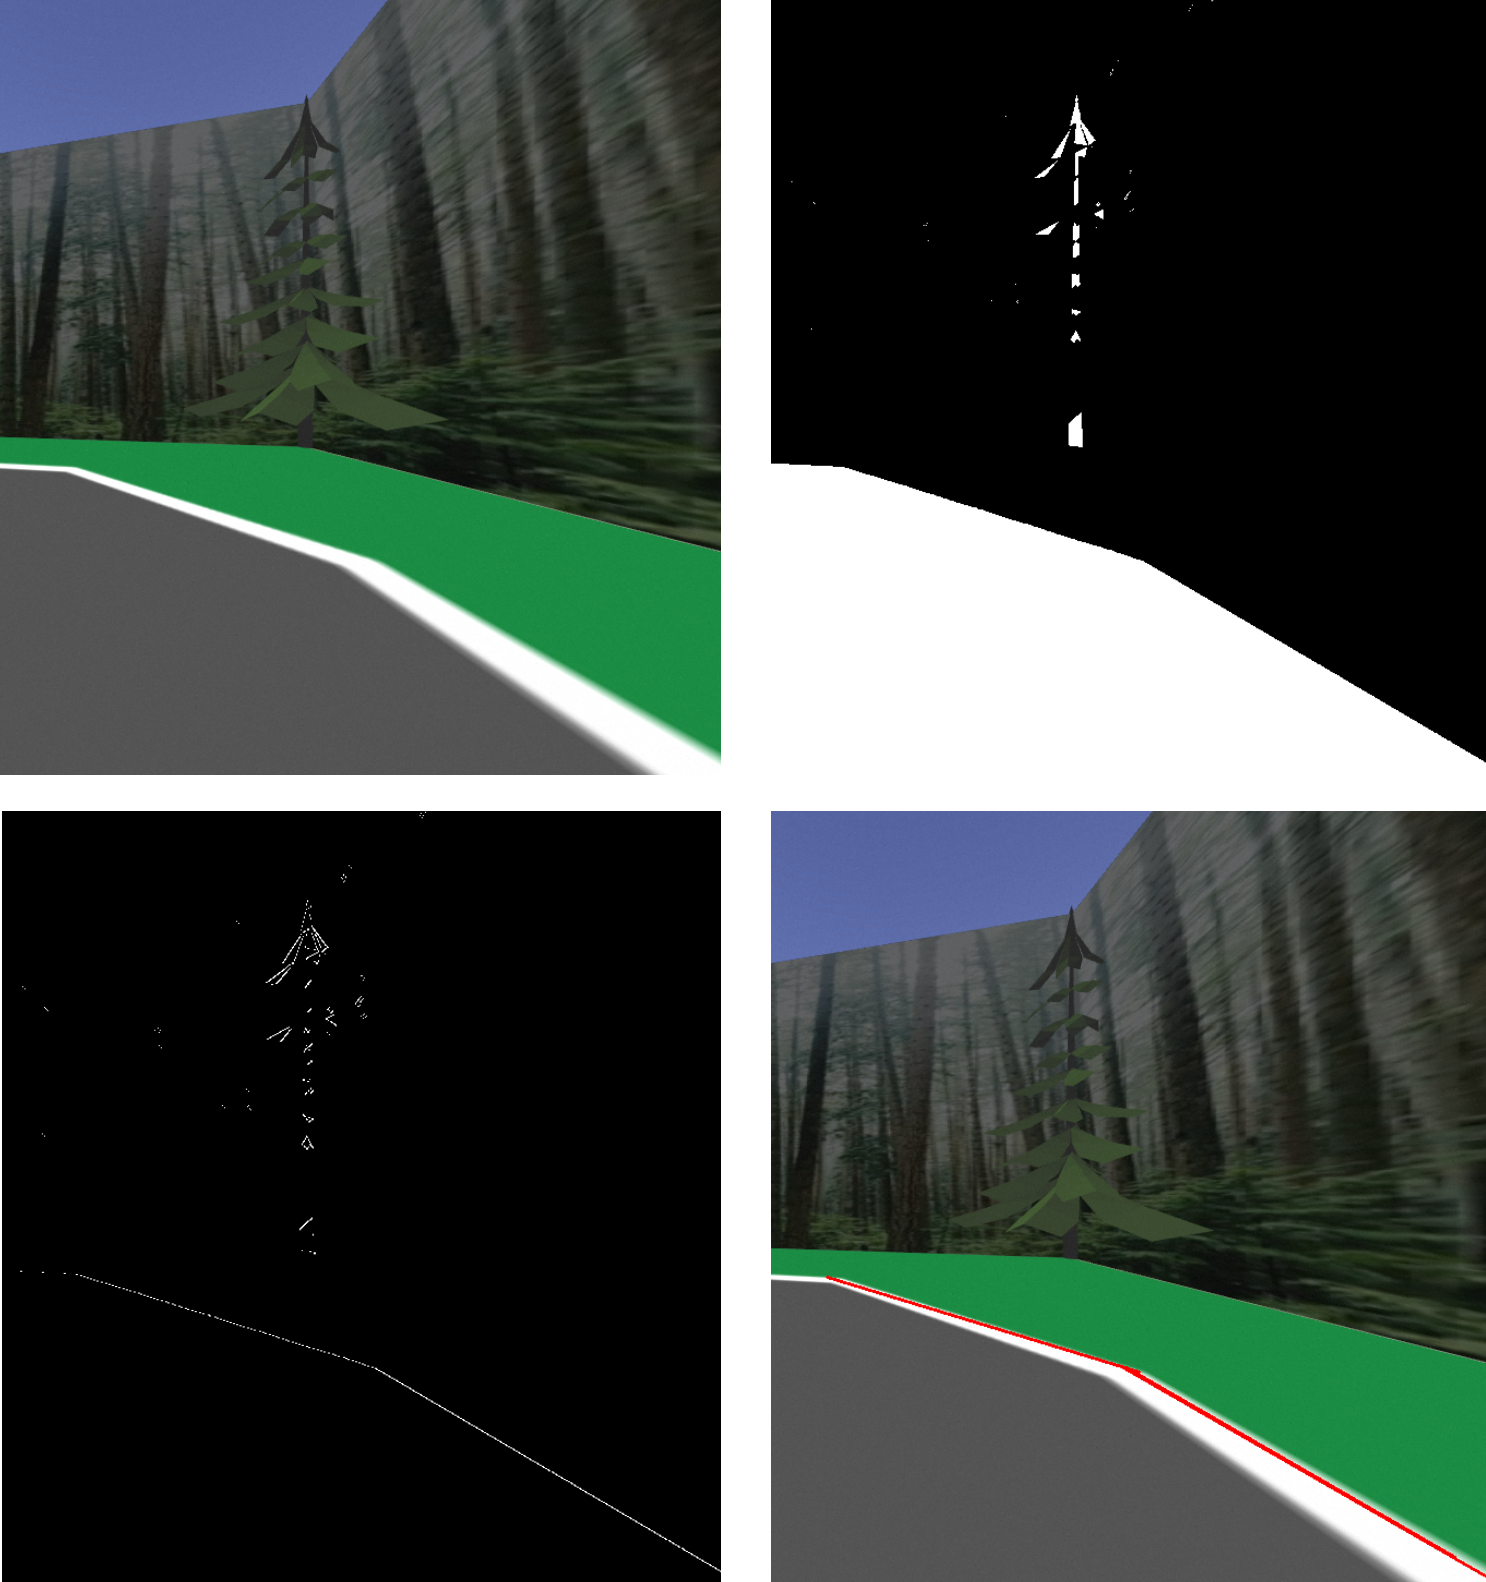
\includegraphics[width=0.7\linewidth]{lines.png}
                \caption{Major steps in pavement line following. Left-to-right, top-to-bottom: Input image; thresholding, line-finding, output lines}
                \label{fig:pavelinefollow}
            \end{figure}

        \subsubsection{Grass Navigation}

            Grass navigation was accomplished with a similar, but more simple pipeline than was used in the pavement navigation, shown in Figure~\ref{fig:grasspipeline}. However, instead of attempting to create lines that fit the edges of the track, we instead use thresholding and other classical techniques to simply isolate the pixels that match the colour of the lines, and then find the average position of the right line. 
            
            A key step in being able to do this was to pass all frames through a brightening step that brings all images up to a standard contrast, as frames from the camera vary in contrast over different areas of the grassy section. Sobel edge detection is also used as a final step to reduce the impact of any large blocks of pixels in the final image other than the line, as they will only contribute an outline's worth of pixels, rather than the entire block. 

            \begin{figure}
                \begin{center}
                    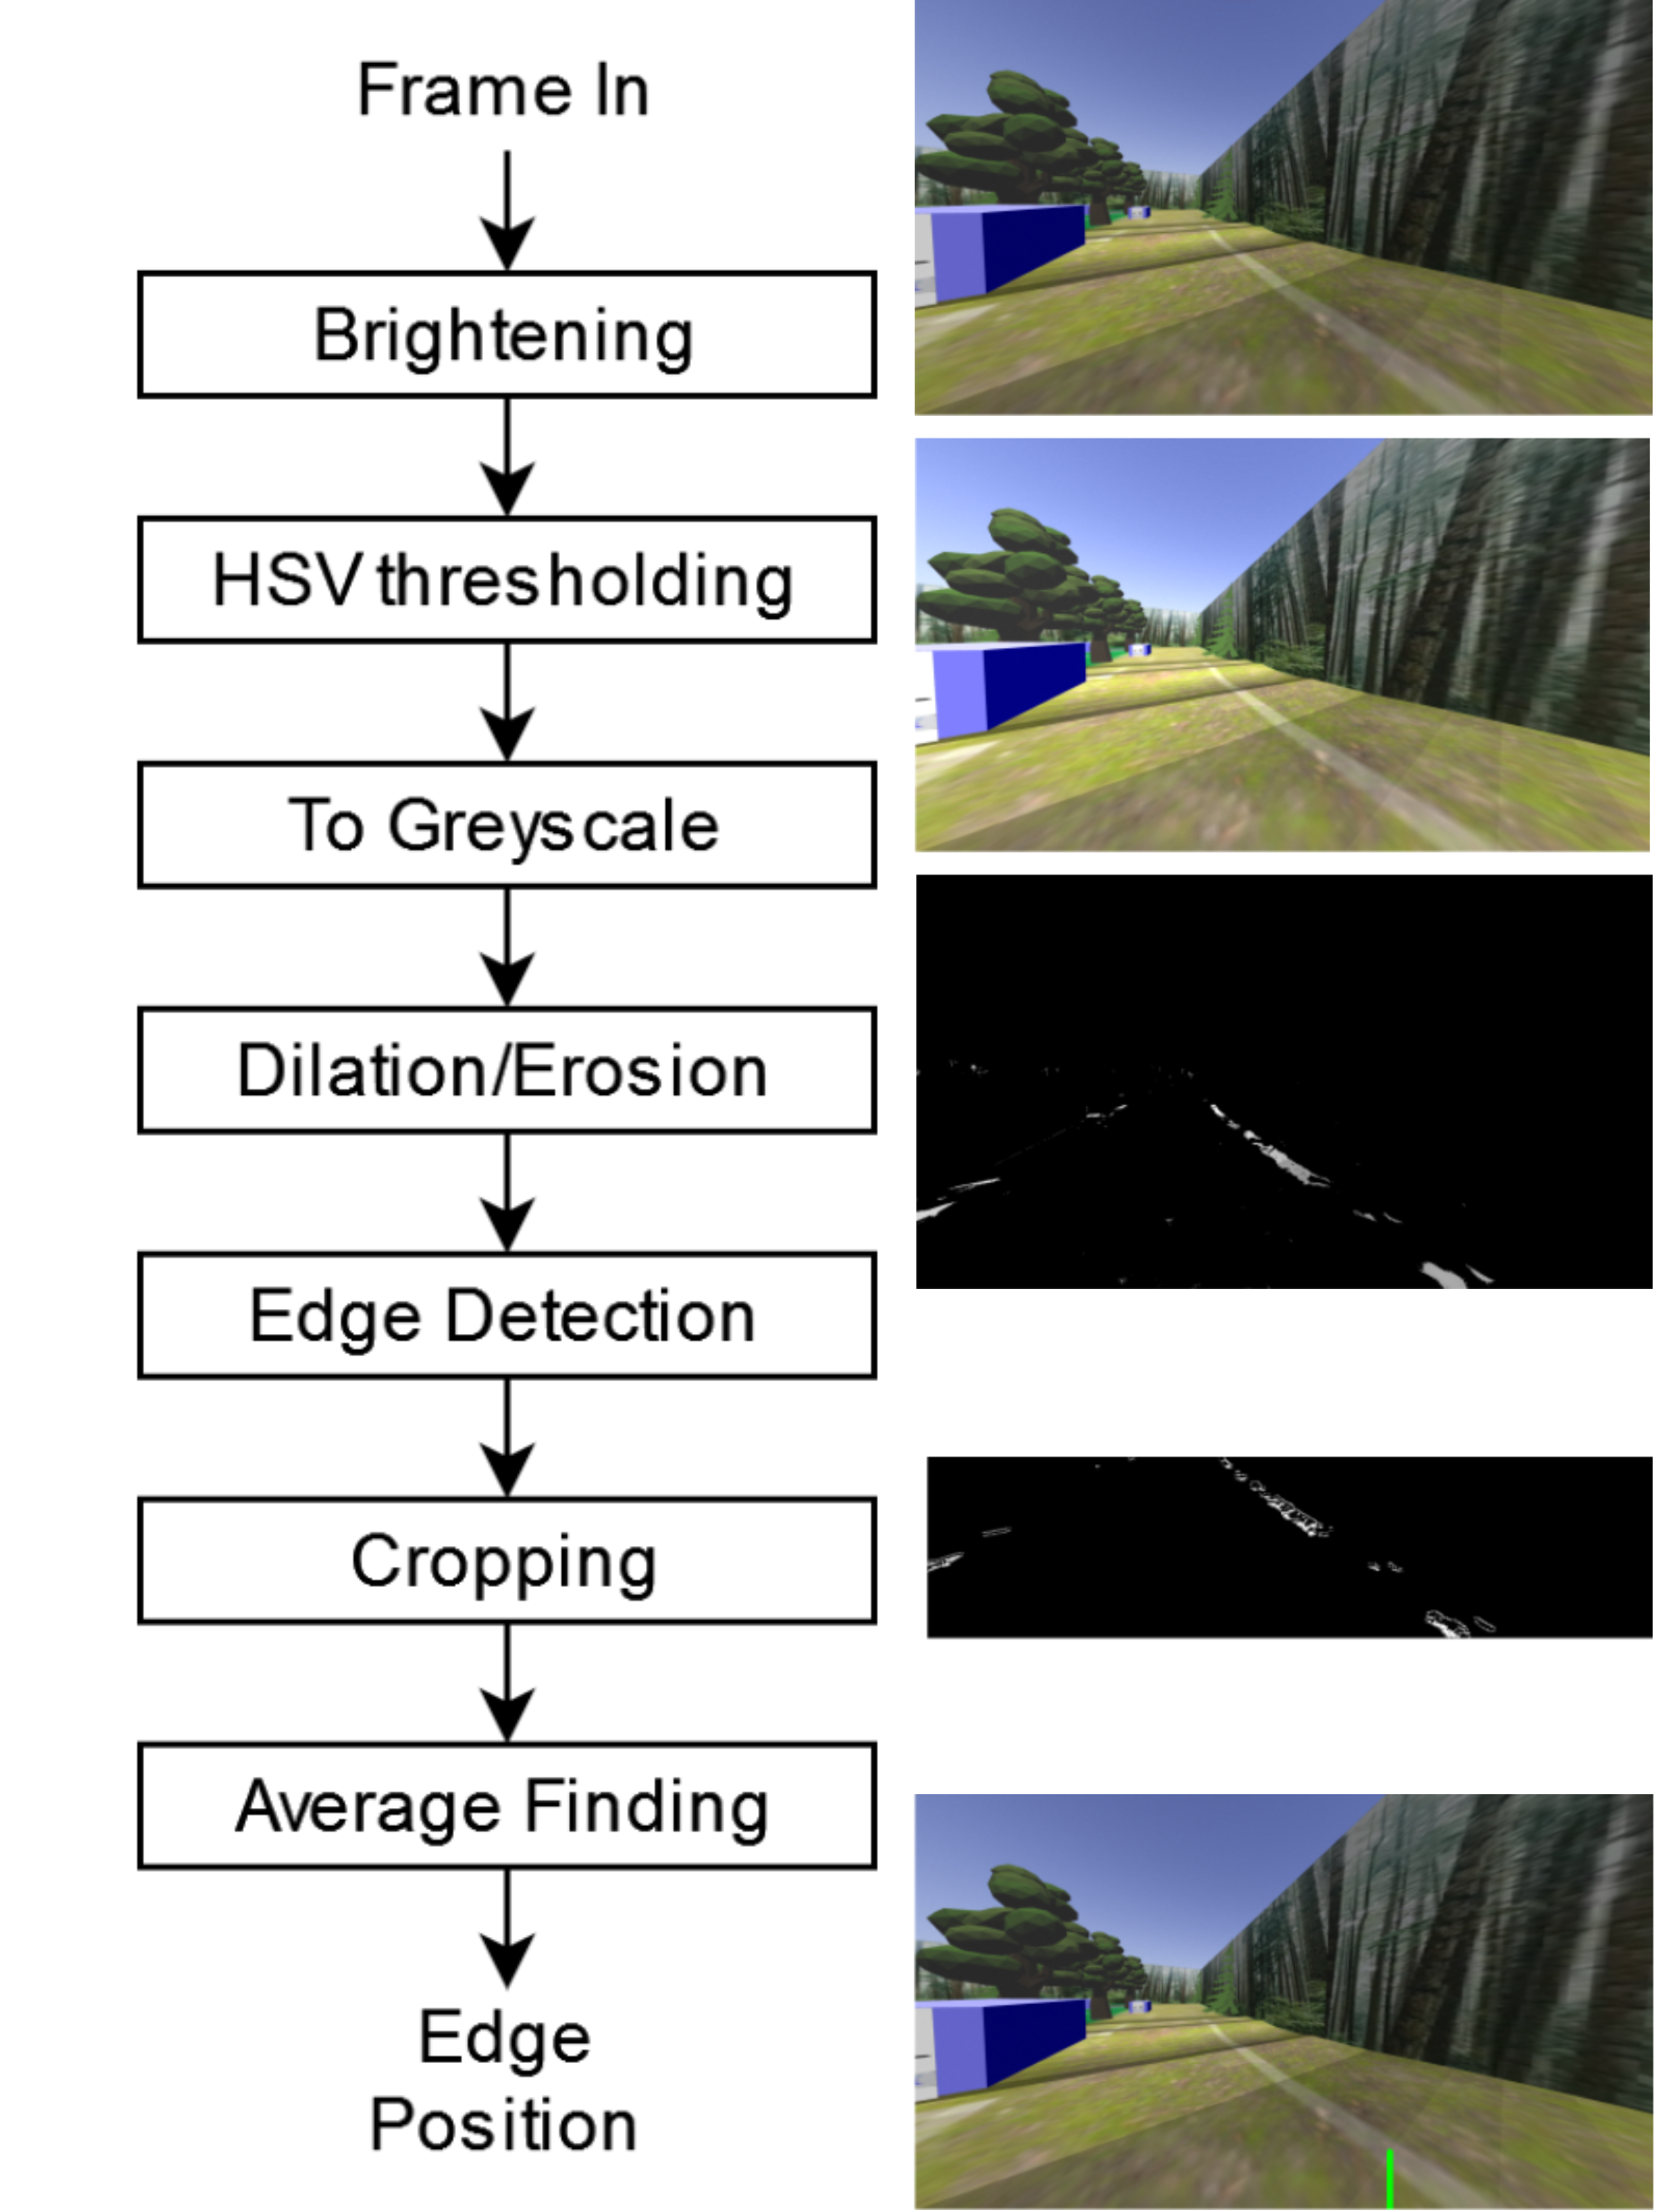
\includegraphics[width=0.5\linewidth]{grass-photos.png}
                \end{center}
                \caption{Grass edge detection image processing pipeline. Key steps shown, from top to bottom, are the input image, brightening, HSV thresholding, cropping and edge detection, and final output.}
                \label{fig:grasspipeline}
            \end{figure}

    \subsection{Plate Reader Commands} \label{platereadercontrol}

    An item noticed during development was that while driving could be stable at relatively high speeds, good readings of the plates would require a more conservative pace. This constraint was mediated by receiving a set of commands from the plate reader node. Whenever the plate reader would detect a plate that we do not have a sufficient number of good readings on, it would send a command to the controller to move into a StopTurn{Left/Right} state. The state machine will save the state it is currently in, and do as commanded by the plate reader for a specified period of time or until commanded to drive again, in which case it will return from whence it came. This additional functionality allowed the system to navigate at a significantly faster pace without missing specific plates.


\section{License Plate Detection}

Plate detection was accomplished using a series of handcrafted filters to extract the individual plate character bounding boxes. This gave a high degree of control over the output, and allowed us to easily tune the system to work on the specific plates used in the competition. The pipeline is shown in Figure~\ref{fig:platepipeline}. Within the plate reader there also exists a tracking system for the predicted plates that ensures our most confident predictions are reported to the license plate topic.

\begin{figure}
\centering
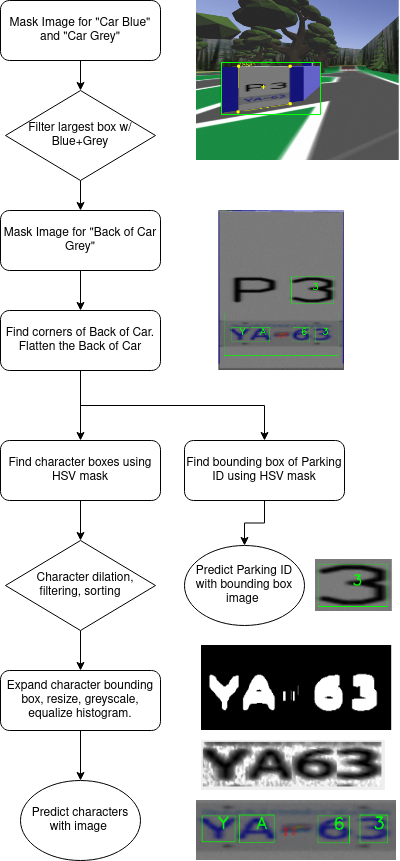
\includegraphics[width=0.9\linewidth]{Image Processing Algorithm.drawio.png}
\caption{Image Processing Algorithm}
\label{fig:platepipeline}
\end{figure}

\subsection{Plate Identification Algorithm}

The first step in the pipeline is to mask the image with a blue and a grey HSV filter to isolate the areas that likely contain cars. These two masks are joined and then contoured. Each contour is checked to see if it contains both blue and grey, otherwise it is discarded (this ensures that only actual cars are investigated further, and not sections of the sky or pavement). 

The largest contour in the image moves onto the next stage of analysis. The contour's bounding box image is masked with a more specific grey HSV filter to get the top and bottom sections of the back of the car. These contours are combined and then fitted to a low quality polygon. The longest 4 lines of the polygon are selected and the intersections of each of the lines found. The four points that are closest to the centroid of the original contour are selected as the corners of the back of the car. Finally, these corners are used to flatten the back of the car and resize it to a standard dimension.

\begin{figure}
\centering
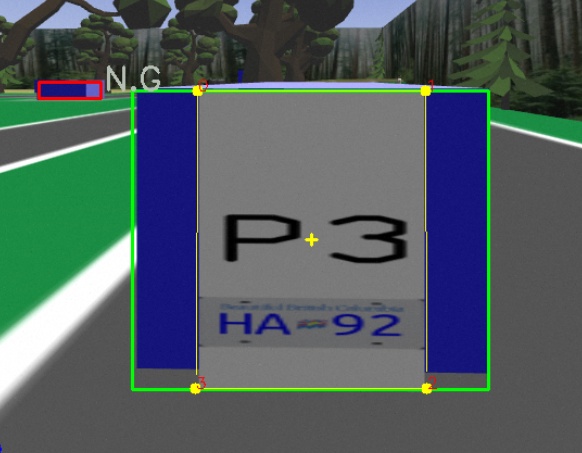
\includegraphics[width=0.8\linewidth]{Annotated back car.png}
\caption{Annotated Back Car. Yellow lines from polygon, yellow dots are the corners, cross is centroid of contour.}
\label{fig:annotatedbackcar}
\end{figure}

The parking ID is extracted using a simple HSV filter, and then greyscaled before passing into the parking ID neural network.

The image is then masked with a blue HSV filter to isolate the license plate characters. This mask undergoes a slight dilation along x and y, then an aggressive dilation only along y. This was chosen to provide a balance of getting the full character without merging large characters into each other. 

\begin{figure}
\centering

\includegraphics[width=0.8\linewidth]{XX00 mask.png}
\caption{Example mask showing non-merging of wide XX combination.}
\label{fig:XX00mask}
\end{figure}

Finally, this mask is contoured, bounding boxed, and then the bounding box expanded. The characters are then filtered based on size and aspect ratio. The remaining contours are then sorted by x position and the characters are extracted from the plate. The characters are then resized to a standard dimension and passed to the neural network for classification.

\begin{figure}
\centering
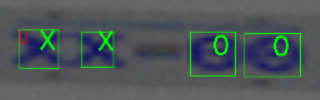
\includegraphics[width=0.8\linewidth]{XX00 identified.png}
\caption{Identified XX00 plate.}
\label{fig:XX00identified}
\end{figure}

\subsection{Neural Networks}

The plate identification algorithm uses a total of 3 neural networks. One to identify the parking ID, one for the plate letters, and one for the plate numbers. Separate networks were chosen for each of these tasks since it simplified the training process and decreased computation time. 

\subsubsection{Parking ID model}

The parking ID model was trained on a dataset of 400 parking IDs extracted from the simulation environment and manually labelled. There was very little optimization put into this network since it was not found to be a bottleneck, and was extremely reliable with a small set of data.

\begin{figure}
    \begin{tabularx}{0.9\linewidth}{ 
         >{\raggedright\arraybackslash}X 
         >{\raggedright\arraybackslash}X 
         >{\raggedleft\arraybackslash}X  }

         Layer (type) & Output Shape & Num. Params. \\ 
        \hline \\
        Conv2D & (None, 48, 48, 3) & 30 \\  
        MaxPool & (None, 24, 24, 3) & 0 \\
        Conv2D & (None, 22, 22, 64) & 1792 \\ 
        MaxPool & (None, 11, 11, 64) & 0 \\
        Flatten & (None, 7744) & 0 \\
        Dropout & (None, 7744) & 0 \\
        Dense & (None, 128) & 991360 \\
        Dense & (None, 8) & 1032 \\
    \end{tabularx}
    \caption{Summary of parking ID neural network}
    \label{fig:parkingidmodel}
\end{figure}

\subsubsection{Plate Letters}

The plate letters model was trained on a dataset of 17000 plate character images extracted from the simulation environment and automatically labelled using the plate list in the environment. The basis of this model was using the example from the character detection lab, and optimized for accuracy and size. In particular, to deal with angled characters that occasionally occurred on the `SFU hill', a deeper initial convolution layer and larger fully connected layer was used. 

\begin{figure}
    \begin{center}
        \begin{subfigure}{0.5\linewidth}
            \centering
            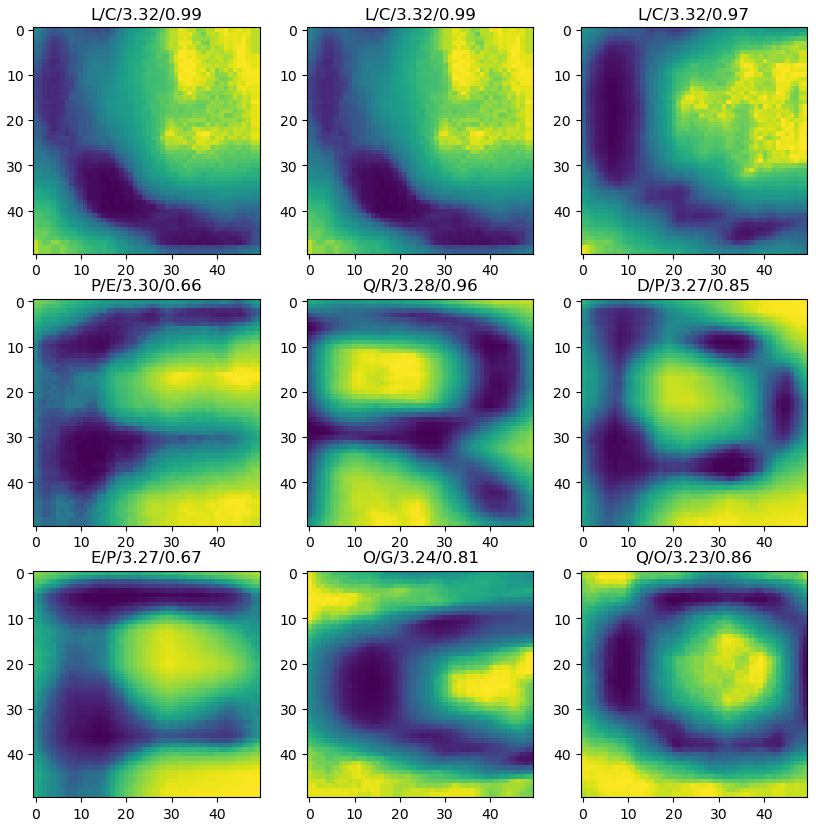
\includegraphics[width=\linewidth]{LetterTopLoss.png}
            \caption{Top Losses}
            \label{fig:lettersloss}
          \end{subfigure}%
          \begin{subfigure}{0.5\linewidth}
            \centering
            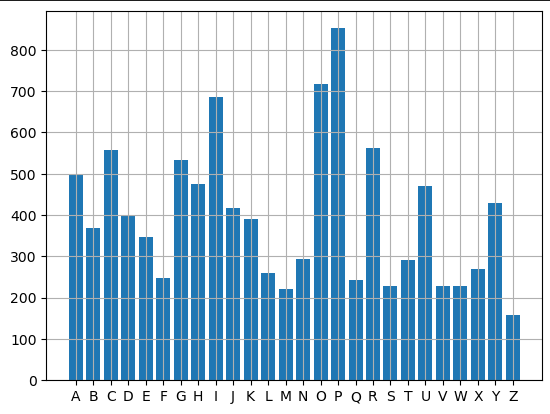
\includegraphics[width=\linewidth]{Letters.png}
            \caption{Dataset}
            \label{fig:letters}
          \end{subfigure}
    \end{center}
    \caption{Top Losses (a) and Dataset (b) for the letter model}
    \label{fig:letters-both}
\end{figure}

\begin{figure}
    \begin{tabularx}{0.9\linewidth}{ 
         >{\raggedright\arraybackslash}X 
         >{\raggedright\arraybackslash}X 
         >{\raggedleft\arraybackslash}X  }

         Layer (type) & Output Shape & Num. Params. \\ 
        \hline \\
        Conv2D & (None, 48, 48, 48) & 480 \\  
        MaxPool & (None, 24, 24, 48) & 0 \\
        Conv2D & (None, 22, 22, 96) & 41568 \\
        MaxPool & (None, 11, 11, 96) & 0 \\
        Flatten & (None, 11616) & 0 \\
        Dropout & (None, 11616) & 0 \\
        Dense & (None, 512) & 5945344 \\
        Dense & (None, 26) & 13338 \\
        
    \end{tabularx}
    \caption{Summary of Plate Letters Model}
    \label{fig:plateletmodel}
\end{figure}

There were many iterations of this network, and it by far required the most amount of tweaking to increase the accuracy without significantly increasing memory size and computation speed. The biggest issue that required resolving was cutting off the edges of letters which could make them appear different. Rather than resolve this on the network side, more optimization was done to the thresholding and extraction system before the network (such as expanding the bounding boxes before passing the letter images into the network). The top losses displayed in Figure \ref{fig:lettersloss} show some of these cut-off letters. After the decision to expand the bounding boxes, much of the most obvious training examples of the cutoff was removed to ensure the network would not be dedicating a significant portion of its size to identifying these obscure edge cases, however the problem was also solved by just piling on tons more new data to make these edge cases more insignificant.

Additionally, the decision to use the greyscale and normalized histogram of the letters was motivated by reducing the size of this network, since it was otherwise requiring over 3x the number of parameters to get reasonably accurate values. 

\subsubsection{Plate Numbers}

The plate numbers model was trained on a dataset of 17000 images of plate characters extracted from the simulation environment and automatically labelled using the plate list in the environment. This model is very similar in structure to the letter network, but smaller since the number of characters to identify is much lower. 

\begin{figure}
    \begin{tabularx}{0.9\linewidth}{ 
         >{\raggedright\arraybackslash}X 
         >{\raggedright\arraybackslash}X 
         >{\raggedleft\arraybackslash}X  }

         Layer (type) & Output Shape & Num. Params. \\ 
        \hline \\
        Conv2D & (None, 48, 48, 16) & 160 \\  
        MaxPool & (None, 24, 24, 16) & 0 \\
        Conv2D & (None, 22, 22, 32) & 4640 \\
        MaxPool & (None, 11, 11, 32) & 0 \\
        Flatten & (None, 3872) & 0 \\
        Dropout & (None, 3872) & 0 \\
        Dense & (None, 256) & 991488 \\
        Dense & (None, 10) & 2570 \\
        
    \end{tabularx}
    \caption{Summary of Plate Numbers Model}
    \label{fig:platenummodel}
\end{figure}

The top losses for this network also tend to consist of characters that have not been correctly extracted from the environment, and improvements to the extraction algorithm reduced the frequency of these errors. 

\begin{figure}
    \begin{center}
        \begin{subfigure}{0.5\linewidth}
            \centering
            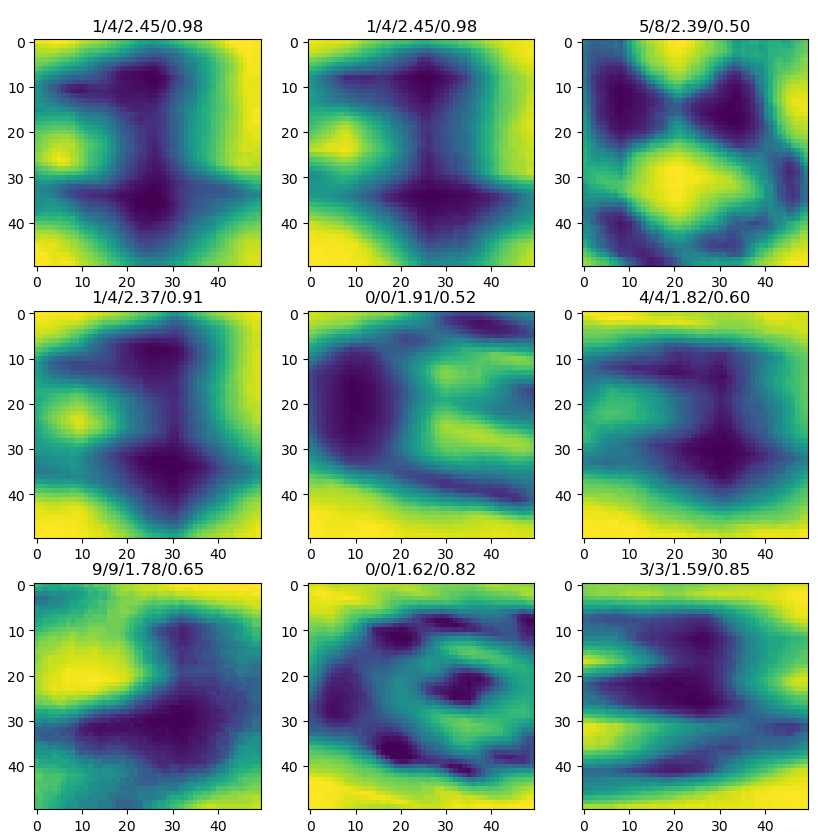
\includegraphics[width=\linewidth]{NumTopLoss.png}
            \caption{Top Losses}
            \label{fig:numsloss}
          \end{subfigure}%
          \begin{subfigure}{0.5\linewidth}
            \centering
            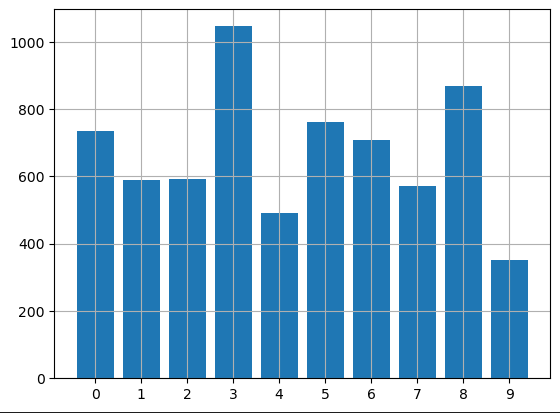
\includegraphics[width=\linewidth]{Numbers.png}
            \caption{Dataset}
            \label{fig:numbers}
          \end{subfigure}
    \end{center}
    \caption{Top Losses (a) and Dataset (b) for the number model}
    \label{fig:numbers-both}
\end{figure}

\subsection{Data Collection} \label{platedata}

The data collection process was conducted entirely using the simulation environment and automated as much as possible. This was chosen to get the most consistent data possible, and minimize the likelihood of a harsh transition from generated to true data. The first stage of collection was to get an identification network working mostly accurate, then secondly add more data on characters that were misidentified. In the first stage, the simulation was run, and all character images collected and labelled (using the plate CSV file in the simulation configuration file). 

A shell script was written to automatically start, run, and stop the simulation and controllers, so that data collection could run autonomously. (See the utilities \href{https://github.com/nvanrumpt/robot_controller_utils2/blob/master/scripts/repeat_runsim.sh}{Github repo} for the script.) Once a sufficient quantity of images were collected, the networks were trained and integrated into the plate reader. In the second stage, only the characters that were misidentified were collected. The process of collecting error images, retraining, and running again was conducted until misidentifications became acceptably infrequent.

\subsection{Performance}

Utilizing the data collection tools talked about in section~\ref{platedata}, the accuracy of the overall algorithm was tracked with the motivation of improving the system. Over the course of 40 runs, reading about 4000 characters, the algorithm only misidentified 10 - giving it an estimated accuracy of 99.8\%. However, even with these errors, the system boasted a {\bf perfect} correct plate reporting record as in all cases there were more correct readings of the plate to outweigh the error. This stellar performance does indicate some simplification could be possible for the networks, but with the amount of time remaining for the project, further changes to the system was not desired.

\subsection{Controller Communication}

At speeds above 0.4~m/s it was noted that the plate reader tended to only receive a single clear frame to get a reading on the plate. To drive at higher speeds, a link between the plate reader and the navigation node was added. Whenever the plate reader gets a good reading on a plate, it sends a command to the controller to stop and turn in the direction of the plate. This ensures that even when driving quickly, the reader gets a sufficient number of readings at each parking ID to be confident in the corresponding plate. 

The plate reader also sends a `done' command to the controller when the final plate has been read confidently. Ideally this would be sent once a good reading had been done on all the plates, but that would require an inner-loop to outer-loop transition, and with limited time, this was neglected in favor of relying on reading all the plates correctly in the first pass. For more details on the controller side of this communication, see section \ref{platereadercontrol}.

\section{User Interface}

The user interface is a simple PyQT5 application to display the relevant information from the simulation and controllers. This application makes it easy to see the current state of the simulation and the controllers, to start and stop the controllers, as well as debugging issues that may arise. The user interface code can be found on GitHub at \href{https://github.com/nvanrumpt/353RobotCompetitionGUI}{nvanrumpt/353RobotCompetitionGUI}.

\begin{figure}
\centering
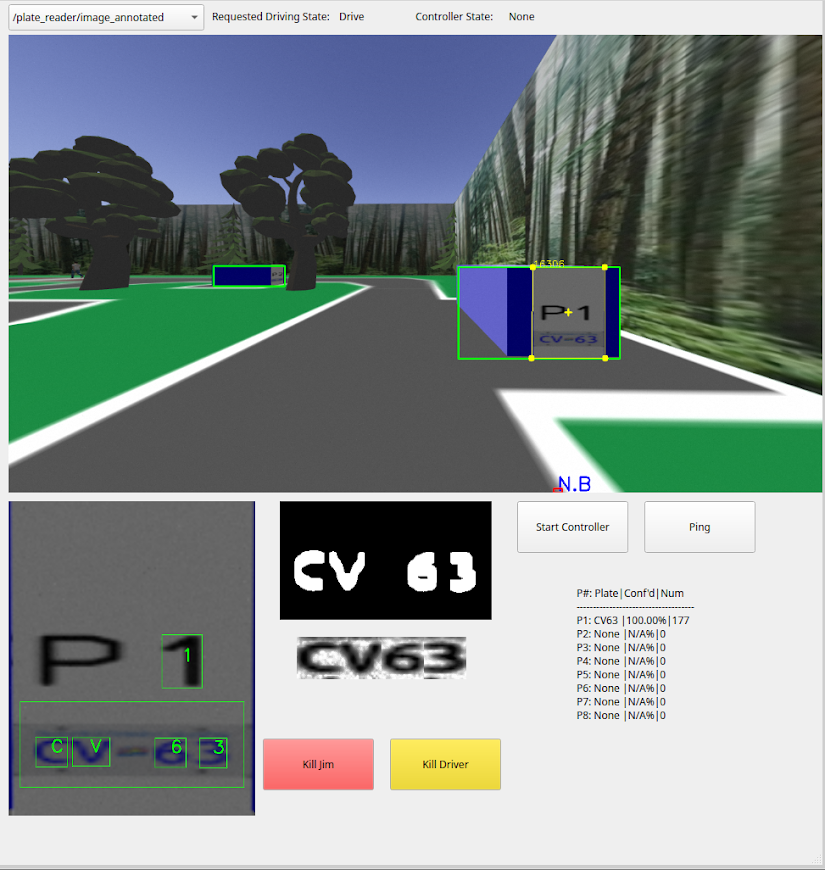
\includegraphics[width=0.8\linewidth]{Gui.png}
\caption{User Interface showing the annotated image from the plate reader.}
\label{fig:UI}
\end{figure}

The largest window can display any image that is published by a node. Most commonly these are the annotated debug images from the plate reader, the navigation node, and the pedestrian/car detector. There is a subscriber bound to each of the image topics that will update the displayed image (if it is the one selected by the dropdown). Each image is resized to match the dimensions of the image label in the UI to ensure that the display is consistent and can be adjusted without regard for the format of the incoming images.
To add additional images, one just needs to add the topic name to the dropdown and code a subscriber to the topic.

The bottom of the UI displays the flattened back of the car, the plate mask, and the images that are passed into the plate identification networks. Also shown is the plate list that has been read, with the predicted plates, the number of good readings, and the confidence of the predictions.

The final aspect of the UI are the buttons that allow the user to start the controllers and kill the simulation. This is useful to ensure that no processes are running headless in the background that will interfere with the next simulation being started. 

\section{Conclusion}

An autonomous driving and plate identification system was created to control a simulated robot within a streetscape environment to collect license plates off parked cars. The driving system was accomplished using primarily classical techniques, and the plate reading also utilizing as much filtering as possible to lighten the neural network computation requirements. This project provided significant hands-on experience with machine learning, ROS, gazebo, and development of custom tools to monitor and improve the algorithms being developed. 

In competition this system performed well - with a perfect score and a time of 56 seconds (4th fastest in the class). Further work could have been done to increase driving speed and lower computation requirements within the plate detection system, however within the time constraints for the competition, the system performed admirably. 

\end{document}